\chapter{Description of the effect of perturbative fields on arcs}

Insert a motivation

\section{Pseudo-Elliptical Models}
The Pseudo-Elliptical models come from the distortion of the lensing potential,
in which
the radial coordinate $r$ is replaced by $\xi$, i.e $\phi(r)\rightarrow
\phi(\xi)$, where
\bea
\xi &=&r_0\,x_\eta=r_0\sqrt{x^2_{1\eta}+x^2_{2\eta}} \label{pe_cord} \\
x_{1\eta}&=&\sqrt{\ae} x_1\\
x_{2\eta}&=&\sqrt{\be} x_2
\eea
where $r_0$ is a model-dependent scaling parameter, and $\ae$, $\be$ are axes
lengths for different parameterizations of the ellipticity.

The most common parameterizations for the ellipticity are

\begin{eqnarray}
\ae=1-\eta &\qquad& \be =1+\eta \label{par_gk}
\end{eqnarray}

and

\begin{eqnarray}
\ae=1-\eta &\qquad & \be =\dfrac{1}{1-\eta} \label{par_gen}
\end{eqnarray}
where \eqref{par_gk}) corresponds to the parametrization of the
Angle Deflection Model ($\eta=\varepsilon$ following the notation of 
\cite{golsekneib})
and \eqref{par_gen}),  corresponds to the standard parametrization
($\eta=\varepsilon_\varphi$
following the notation of \cite{meneg}).

Working in polar coordinates $x_1=x\cos{\te}$ , $x_2=x\sin{\te}$ we obtain

\beq
\xi=r\sqrt{\ae \cos^2{\te}+\be\sin^2{\te}}.
\label{pe_radius}
\eeq

Regarding the Perturbative Approach, we can write any Pseudo-Elliptical Model as

\beq
\phi_{_\mathrm{PE}}(r)=\phi_0(r)+\phi(\xi)-\phi_0(r), \quad
\psi_{_\mathrm{PE}}(r)=\phi(\xi)-\phi_0(r).
\label{pe_model}
\eeq

Here, we use the following notation

\begin{eqnarray*}
\phi_\xi\equiv \phi(\xi), &\quad&  \phi^\prime_\xi \equiv
\dfrac{d\phi(\xi)}{d\xi}, \quad \phi^{\prime\prime}_\xi \equiv
\dfrac{d^2\phi(\xi)}{d\xi^2}\\
\phi_0\equiv \phi(r),&\quad&  \phi^\prime_0 \equiv \dfrac{d\phi(r)}{dr}\\
\xer \equiv \re \sqrt{\ae \cos^2{\te}+\be\sin^2{\te}},&\quad&
\scriptg(\eta,\te)=\re^2\mathcal{A}(\eta)\sin{(2\te)},\quad
\mathcal{A}(\eta)=\be-\ae
\end{eqnarray*}

Now we derive the analytical expression for the main fields of the
Perturbative Method. Using the definition, we have

\beq
f_0(\te)=\phi(\xer)-\phi_0(\re)
\eeq
The derivative of $f_0$ with respect to $\te$ is
\beq
\frac{df_0}{d\te}=\dfrac{d\phi_{\xer}}{d\xer}\dfrac{d\xer}{d\te}=\frac{1}{2}
\dfrac{\phi^\prime_{\xer}}{\xer}\scriptg(\eta,\te)
\label{df0_pe}
\eeq
where, we used 
\beq
\dfrac{d\xer}{d\te}=\frac{1}{2}\dfrac{\scriptg(\eta,\te)}{\xer}.                
\label{dxer_pe}
\eeq

From Eqs.{(\ref{pe_radius}, \ref{pe_model})} we may obtain 

\begin{equation*}
\dfrac{\prtl \psi_{_{\mathrm{PE}}}(r) }{\prtl
r}=\dfrac{d\phi_\xi}{d\xi}\dfrac{\prtl \xi}{\prtl r}-\dfrac{\prtl \phi_0}{\prtl
r}
\end{equation*}

Evaluating this at the Einstein Radius, we have
\beq
f_1(\te)=\dfrac{\xer}{\re}\phi^\prime_{\xer}-\phi^\prime_0
\label{f1_pe}
\eeq

Also, taking the derivative of Eq.~(\ref{df0_pe}) respect to $\te$, it is
straightforward to get
\beq
\dfrac{d^2f_0}{d\te^2}=\frac{1}{2}\scriptg_\te(\eta,\te)\dfrac{\phi^\prime_{\xer
}}{\xer}+%
\frac{1}{4}\left[
\dfrac{\scriptg(\eta,\te)}{\xer}\right]^2\left(\phi^{\prime\prime}_{\xer}-\dfrac
{\phi^{\prime}_{\xer}}{\xer}  \right)
\label{ddf0_pe}
\eeq
where $\scriptg_\te(\eta,\te)\equiv d\scriptg(\eta,\te)/d\te$.

Now, to write the expression of $d^nf_0 \over d\te^n$ and $f_1$ as function of
the lensing functions, we use some basic relationships valid for
any circular model

\bea
\phi^\prime &\equiv& \dfrac{d\phi(r)}{d r}=\alpha(r) \label{dphi}\\
\phi^{\prime\prime}&\equiv& \dfrac{d^2\phi(r)}{d
r^2}=2\kappa(r)-\dfrac{\alpha(r)}{r}\label{ddphi}\\
\gamma(r)&=&\dfrac{\alpha(r)}{r}-\kappa(r) \label{shear_gen}
\eea

Using these relationships and $r$ is a dummy variable, we have for the main
fields
\bea
\dfrac{df_0}{d\te}&=& \frac{1}{2}\dfrac{\alpha(\xer)}{\xer}\scriptg(\eta,\te)
\label{df0_pe2}\\
f_1(\te)&=&\dfrac{\xer}{\re}\alpha(\xer)-\alpha(\re) \label{f1_pe2}
\eea
and further
\beq
\label{ddf0_pe2}
\dfrac{d^2f_0}{d\te^2}=\frac{1}{2}\scriptg_\te(\eta,\te)\dfrac{\alpha(\xer)}{
\xer}-%
\frac{\gamma(\xer)}{2}\left[ \dfrac{\scriptg(\eta,\te)}{\xer}\right]^2 .
\eeq

\subsection{Expression for small values of the ellipticity}

Now, we expand the analytical expressions for the main fields 
Eqs.(\ref{df0_pe2}, \ref{f1_pe2}) in a Taylor Series around $\eta=0$. 
Is straightforward to verify that

\bea
\dfrac{df_0}{d\te}& \approx & \eta\alpha(\re)\re\sin{(2\te)}
\label{df0_pe_appr}\\
f_1(\te)&\approx&-\eta \kappa(\re)\re\cos{(2\te)} \label{f1_pe_appr}
\eea

And from  Eq.~(\ref{df0_pe_appr}), or expanding Eq.~(\ref{ddf0_pe2}) in a Taylor
Series, we obtain
to
\beq
\dfrac{d^2f_0}{d\te^2}=2\eta\alpha(\re)\re\cos{(2\te)} \label{ddf0_pe_appr}
\eeq

For example, if we consider the Pseudo-Elliptical SIS (setting $\re=1$) we get
to the
Eqs.(17) of Alard's Paper 2008 (without considering the contribution of
substructures), i.e,
\begin{eqnarray*}
 f_1(\te)&\approx&-\frac{\eta}{2}\cos{(2\te)}\\
 \dfrac{df_0}{d\te}& \approx & \eta\sin{(2\te)} 
\end{eqnarray*}
 


\pagebreak

\section{Elliptical Models } % Bruno
\subsection{General results for elliptical models}
Contrary to pseudo-elliptical models, elliptical models introduce the
ellipticity directly into the convergence. To do this, we apply the following
transformation to the convergence of an axisymetric model:
\beq
\label{variavel-eliptica}
x^2 \rightarrow \frac{x^2}{a^2} + \frac{y^2}{b^2}.
\eeq
It can then be shown that the derivatives of the potential in Cartesian
coordinates can be written as (cf. Gabriel's master thesis):
\begin{eqnarray}
\label{der-pot1}
\phi_1(x_1,x_2) &=& abx_1J_0, \\
\label{der-pot2}
\phi_2(x_1,x_2) &=& abx_2J_1, \\
\label{der-pot3}
\phi_{11}(x_1,x_2)&=& 2abx_1^2K_0 + abJ_0, \\
\label{der-pot4}
\phi_{22}(x_1,x_2)&=& 2abx_2^2K_2 + abJ_1, \\
\label{der-pot5}
\phi_{12}(x_1,x_2)&=& 2abx_1x_2K_1,
\end{eqnarray}
where $\phi_i$ is the derivative of $\phi$ according to $x_i$ and $J_n$ and
$K_n$ are defined as  
\begin{eqnarray}
J_n(r,\te)&=& \int_{0}^{1} \dfrac{\kappa\left( m(u) \right) }{\left[1-(1-b^2)u
\right]^{\frac{1}{2}+n} \left[1-(1-a^2)u \right]^{\frac{3}{2}-n}}du,\label{Jn}\\
K_n(r,\te)&=& \int_{0}^{1} \dfrac{u\kappa'\left( m(u) \right) }{\left[1-(1-b^2)u
\right]^{\frac{1}{2}+n} \left[1-(1-a^2)u \right]^{\frac{5}{2}-n}}du,\label{Kn}
\end{eqnarray}
In these integrals, $m$ is written as (in radial coordinates for our purposes)
\beq
m^2 = ur^2\left( \dfrac{cos^2\te}{1-(1-a^2)u} +
\dfrac{sen^2\te}{1-(1-b^2)u}\right)\,.\label{m}
\eeq
From the first-order derivatives in Cartesian coordinates, we can obtain the
ones in polar coordinates using the transformation of the gradient
\bea
\frac{\partial\phi}{\partial r}&=&\phi_1\cos\,\te+\phi_2 \sin\,\te\\
\frac{\partial\phi}{\partial \te}&=&-\phi_1\sin\,\te+\phi_2\cos\,\te
\eea
Then it is easy to obtain
\bea
\frac{\partial \phi}{\partial
r}&=&abr\left[J_0(r,\te)cos^2\te+J_1(r,\te)sin^2\te\right]\\
\frac{\partial \phi}{\partial \te}&=&abr^2sin\,\te
cos\,\te\left[J_1(r,\te)-J_0(r,\te)\right]
\eea
In order to get the coefficients in Alard's expansion, we need to extract the
axisymmetric part of the potential. Defining
$\psi(r,\te)\equiv\phi(r,\te)-\phi_0(r)$, we arrive at
\bea
f_1&=&\re\left[ab\left(J_0(R_E,\te)\,cos^2\te+J_1(R_E,\te)\,sen^2\te\right)-1\right]\label{f1-sie}
\\[10pt]
\frac{{\rm d}f_0}{{\rm
d}\te}&=&ab\,\frac{\re^2}{2}\left[J_1(R_E,\te)-J_0(R_E,\te)\right]sen\,2\te\label{df0-sie}\\[10pt]
\frac{{\rm d}^2f_0}{{\rm
d}\te^2}&=&ab\,\re^2\Bigg\{\left[J_1(R_E,\te)-J_0(R_E,\te)\right]cos\,2\te +\nonumber\\ 
&&+\frac{\re^2}{2}\left[K_0-2K_1(R_E,\te)+ K_2(R_E,\te)\right]sen^22\te\Bigg\}\label{d2f0-sie}
\eea
\subsection{SIE: CC, caustics and deformation cross-section}

SIE models are the elliptical generalization of the SIS model. As such, the
convergence can be obtained using eq. (\ref{variavel-eliptica}):
\beq
\kappa_{SIE}(m)=\frac{R_E}{2m}\label{convergence-SIE}
\eeq
where $m$ is given by eq. (\ref{m}). In this case, it is possible to calculate
the integrals (\ref{Jn}) and (\ref{Kn}) analitically.
\beq
J_n(r,\te)=\frac{R_E}{r}\frac{1}{\sqrt{\varepsilon_n+A(\theta)}}\tanh^{-1}
\left(\sqrt{\frac{\varepsilon_n+A(\theta)}{1+A(\theta)}}\right)
\eeq
where
\bea
\varepsilon_0&=&1-a^2\\
\varepsilon_1&=&1-b^2\\
A(\theta)&=&b^2-1+(a^2-b^2)\cos^2\theta
\eea
It will be useful to express eqs. (\ref{Jn}) and (\ref{Kn}) in terms of the
ellipticity. Let us choose the prescription
$\left(a=(1-\epsilon)^{-1/2},\,b=(1-\epsilon)^{1/2}\right)$. Then
\bea
\bar{\varepsilon}_0&=&\frac{\epsilon}{\epsilon-1}\\
\bar{\varepsilon}_1&=&\epsilon\\
\bar{A}(\theta)&=&\epsilon\left[-1+\left(\frac{\epsilon-2}{\epsilon-1}
\right)\cos^2\theta\right]
\eea
and
\bea
J_0(r,\te)&=&\frac{\sigma}{r}\left(\frac{\tanh^{-1}\left[\sqrt{\frac{\epsilon^2-\epsilon(\epsilon-2)\cos^2\theta}{\epsilon^2-\epsilon(\epsilon-2)\cos^2\theta-1}}\right]}{\sqrt{\frac{\epsilon^2-\epsilon(\epsilon-2)\cos^2\theta}{\epsilon-1}}}\right)\\
J_1(r,\te)&=&\frac{\sigma}{r}\left(\frac{\tanh^{-1}\left[\sqrt{\frac{2\epsilon^2-2\epsilon-\epsilon(\epsilon-2)\cos^2\theta}{\epsilon
^2-\epsilon(\epsilon-2)\cos^2\theta-1}}\right]}{\sqrt{\frac{2\epsilon
^2-2\epsilon-\epsilon(\epsilon-2)\cos^2\theta}{\epsilon-1}}}\right)\\
K_0&=&\\
K_1&=&\\
K_2&=&
\eea
With these results, we obtain
\bea
f_1&=&\\[10pt]
\frac{{\rm d}f_0}{{\rm
d}\te}&=&\\[10pt]
\frac{{\rm d}^2f_0}{{\rm
d}\te^2}&=&
\eea
For small ellipticity, we can do a series expansion around $\epsilon=0$. At
linear order, this gives
\bea
J_0(r,\te)cos^2\te+J_1(r,\te)sin^2\te&=&\frac{\sigma}{r}\left(1-\frac{
\epsilon\cos\,2\theta}{2}\right)\\
J_1(r,\te)-J_0(r,\te)&=&\frac{2\epsilon}{3}
\eea
and
\bea
f_1&=&\re\left[\frac{\sigma}{r}\left(1-\frac{\epsilon\cos\,2\theta}{6}
\right)-1\right]\\[10pt]
\frac{{\rm d}f_0}{{\rm
d}\te}&=&\re\sigma\frac{\epsilon}{3}\sin\,
2\te\\[10pt]
\frac{{\rm d}^2f_0}{{\rm
d}\te^2}&=&
\eea
\subsection{ENFW: CC, caustics and deformation cross-section}
\section{Substructures}
\begin{wrapfigure}{r}{0.4\textwidth}
  \begin{center}
%  \centering{\epsfig{Fig_subsstructure.eps,width=0.45\textwidth}}
   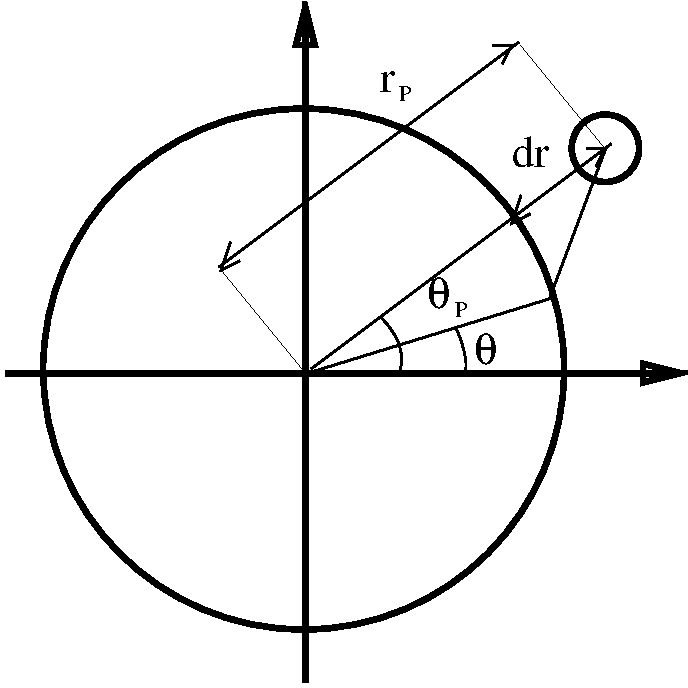
\includegraphics[width=0.30\textwidth]{graphics/Fig_subsstructure.pdf}
\label{fig:substruc}
  \end{center}
    \caption{Geometry of the perturbation induced by the substructure. The large
circle corresponds to Einstein Ring,
  while the smaller one represents the substructure located at $r_p=\re
+\zeta$.}
\end{wrapfigure}

We may consider the perturbation as
\begin{equation}
\psi_{ss}(r,\te,\pi_p)=\varphi(\zeta)
\end{equation}
where the ``ss'' indicates substructure, $\varphi$ corresponds to a central
potential (any circular model, such as SIS, NFW and so on) and $\pi_p$
are the substructure parameters, such as mass, position and inclination angle.
$\zeta$ comes from Fig. \ref{fig:substruc} (in which $dr=\zeta$)
where
\begin{eqnarray}
\vec{r}_p&=&r_p\cos{\tep}\hat{\imath} + r_p\sin{\tep}\hat{\jmath}\\
\vec{r}&=&r\cos{\te}\hat{\imath} + r\sin{\te}\hat{\jmath}\\
\vec{\zeta}&=&\vec{r}_p-\vec{r}.
\end{eqnarray}
Taking the modulus of $\zeta$, is straightforward to verify that
\begin{equation}
\zeta(r,\te)=\sqrt{r^2-2r r_p\cos{(\te-\tep)}+r^2_p}.
\label{xirte}
\end{equation}

Before giving the analytical expression for the fields $f_1$ and ${d^nf_0 \over
d\te^n}$ ($n=1,2$), we
give some useful results (with $\zeta = \zeta(r,\te)$).
\begin{eqnarray}
\Omega(\zeta) & \equiv & r r_p \sin{(\te-\te_p)} \\
\dfrac{d\zeta}{d\te}&=&  \dfrac{\Omega(\zeta)}{\zeta}\\
\dfrac{d\Omega(\zeta)}{d\te}&=&r r_p\cos{(\te-\te_p)}\\
\dfrac{d\zeta}{dr}&=&\dfrac{r-r_p\cos{(\te-\te_p)}}{\zeta}
\end{eqnarray}

Introducing the following notation
\begin{eqnarray}
\varphi_\zeta & \equiv & \varphi(\zeta) \nonumber \\
\varphi^\prime_\zeta &=& d\varphi_\zeta \over d\zeta \nonumber  \\
\varphi^{\prime\prime}_\zeta &=& d^2\varphi_\zeta \over d\zeta^2 \nonumber 
\end{eqnarray}

and using the relations above we have

\begin{eqnarray}
\dfrac{\prtl \psi_{ss}}{\prtl
\te}&=&\Omega(\zeta)\dfrac{\varphi^\prime}{\zeta}\label{df0}\\
\dfrac{\prtl^2
\psi_{ss}}{\prtl\te^2}&=&\left[\varphi^{\prime\prime}_\zeta-\dfrac{
\varphi^\prime_\zeta}{\zeta}\right]%
\left(\dfrac{\Omega(\zeta)}{\zeta}\right)^2+[r
r_p\cos{(\te-\tep)}]\dfrac{\varphi^\prime_\zeta}{\zeta}\label{ddf0}\\
\dfrac{\prtl \psi_{ss}}{\prtl
r}&=&[r-r_p\cos{(\te-\tep)}]\dfrac{\varphi^\prime_\zeta}{\zeta}\label{f1}
\end{eqnarray}

Using the Eqs.~(\ref{dphi}, \, \ref{ddphi} and \ref{shear_gen}), where $r$ is
dummy variable, we can define 
$\al_\zeta=\al(\zeta)=\varphi^\prime_\zeta$, $\kappa_\zeta=\kappa(\zeta)$ and
$\gamma_\zeta=\al_\zeta/\zeta-\kappa_\zeta$. 
From Eqs.(\ref{xirte}, \ref{df0}-\ref{f1}) (evaluated at $r=\re$), we obtain the
analytical expressions for the main fields of
the perturbative approach as function of the angle deflection and convergence,
i.e.
\begin{eqnarray}
\dfrac{df_0}{d\te}&=&\al_{\xie}\dfrac{\Omega(\xie)}{\xie}\\
% \dfrac{d^2f_0}{d\te^2}&=&2\left[\kappa_{\xie}-\dfrac{\al_{\xie}}{\xie}\right]%
% \left(\dfrac{\Omega(\xie)}{\xie}\right)^2+\al_{\xie}\dfrac{[\re
%r_p\cos{(\te-\tep)}]}{\xie}\\
\dfrac{d^2f_0}{d\te^2}&=& \al_{\xie}\dfrac{[\re r_p\cos{(\te-\tep)}]}{\xie}% 
- 2\gamma_{\xie} \left(\dfrac{\Omega(\xie)}{\xie}\right)^2\\
f_1(\te)&=&\al_{\xie}\dfrac{[\re-r_p\cos{(\te-\tep)}]}{\xie},
\end{eqnarray}

\subsection{SIS model as substructure}

As application of these analytical expressions, we will consider the case of the
Singular Isothermal Sphere, for
which $\psi(r,\te,\pi_p)=m_p\zeta$, where $m_p$ is the mass contained within the
critical radius.
Is very easy to verify that $\al_\zeta=m_p$,  $\kappa_\zeta=m_p/(2\zeta)$ (this
expression comes from the usual
definition of the SIS convergence) and therefore we obtain
\begin{eqnarray}
\dfrac{d f_0}{d\te}&=&\dfrac{\re m_p r_p \sin{(\te -\tep)}}{\sqrt{\re^2-2\re
r_p\cos{(\te-\tep)}+r^2_p}}.\\
f_1&=&\dfrac{m_p[\re-r_p\cos{(\te-\tep)}]}{\sqrt{\re^2-2\re
r_p\cos{(\te-\tep)}+r^2_p}}.
\end{eqnarray}
If we choose $\re=1$ we get to the expression given in Alard's 2008 Paper .

Another quantity useful to calculate the critical and caustic lines is
\begin{equation}
\dfrac{d^2 f_0}{d\te^2}=\dfrac{m_p}{\sqrt{\re^2-2\re
r_p\cos{(\te-\tep)}+r^2_p}}%
\left[\re r_p\cos{(\te-\tep)}- \dfrac{[\re r_p\sin{(\te-\tep)}]^2}{\re^2-2\re
r_p\cos{(\te-\tep)}+r^2_p} \right].
\end{equation}

Conclusions: Now, we are able to at least consider substructure in the form of a
circular lens.


\section{External Shear + Continuous Matter}

Objects near the main lens galaxy or along the line of sight often perturb the
lensing potential.
In the case that we are considering the contribution of the mass distribution
external to the lens,
we can work with the potential coming from the external mass + external shear.
\beq
\phi(r)=\phi_0(r)+\frac{r^2}{2}\left[ \kex-\gex\cos{2(\te-\te_\gamma)}\right].
\eeq
where the perturbative potential, in this case is
\beq
\psi_{_{\mathrm{EX}}}(r)=\frac{r^2}{2}\left[
\kappa_{_{\mathrm{EX}}}-\gamma_{_{\mathrm{EX}}}\cos{2(\te-\te_\gamma)}\right]
\eeq
From the expression above, is easy get to
\bea
f_1(\te)&=& \re\left[\kex-\gex\cos{2(\te-\te_\gamma)}   \right]\\
\dfrac{d f_0}{d\te} (\te)&=& \re^2\gex\sin{2(\te-\te_\gamma)}\\
\dfrac{d f^2_0}{d\te^2}(\te)&=& 2\re^2\gex\cos{2(\te-\te_\gamma)}\\
\eea

Note that this model for perturbation is the most simples, but don't forget that
$\re$ depends on the
unperturbed potential, for example: could be NFW, SIS, Cuspy-NFW, etc etc. 
